\chapter{项目要点}


    \section{我们想做什么?}
        \subsection{右手扫弦}
        扫弦是吉他的特色之一,容易上手;结合声乐可以弹唱大部分流行歌曲;对精度要求不高

        \subsection{左手按弦}
        为了能扫出不同和弦,我们需要左手来选择和弦。在普通吉他中,左手用手指在按下六根弦中的\
        不同离散的位置(称为“品”),也可以不按。这样不同的按法,就能让右手扫弦时产生不同的和弦声音。


    \section{右手?算法?挑战性在哪?}
        TODO

        六根弦位置固定

        利用右手的位置、走向、高度等信息

        连续同方向扫弦问题

        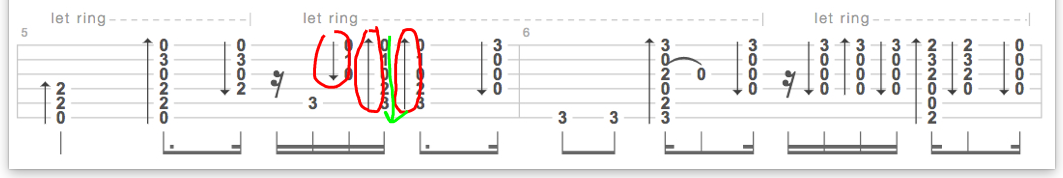
\includegraphics[width=\textwidth]{strumming}

    \section{左手?算法?挑战性在哪?}
        由于该动作手掌朝上,在桌面上放置LM时无法捕捉到左手手指的信息,并且由于空间中没有标\
        “品”的位置,非常容易弹错。因此为了容易上手,我们使用大多数吉他应用app的套路,\
        就是用预设和弦组合,然后以button的形式让用户选择。

        我们选择C调的常用和弦以九宫格的形式呈现给用户,对应到空间中就是一个虚拟的九宫格\
        ,左手用点击来选择和弦。我们用了选择确认反馈提升用户体验。
